\chapter{Diseño de la propuesta}

En este capítulo se va a analizar los requisitos que tiene que tener este proyecto, que se va a abarcar en este trabajo, como va a ser la red de dispositivos que es necesario desplegar, de que tipo son e identificar que tarea va a realizar cada uno de estos nodos.

Para el análisis del escenario que se supone el contacto con un cliente propietario de un invernadero, obteniendo las medidas y el número de nodos necesarios. A partir de ahí se puede realizar un análisis de que es necesario para el despliegue del producto.

Con esta breve introducción, se van a identificar los requisitos que debe cumplir el proyecto. Tras esto se realizarán diferentes diseños para entender la estructura del código y de la red.

\section{Descripción del entorno y análisis de requisitos}

Para empezar, se va a suponer que tenemos un invernadero dividido en diferentes secciones. Estas se establecen en función del radio de actuación de algunos sensores o actuadores. Por lo tanto en cada una debe haber diferentes nodos que son necesarios para cumplir las expectativas y requisitos. Los dispositivos a desplegar se pueden agrupar en los siguientes apartados:

\subsection{Sensores}

En este proyecto y en la mayoría, los datos son la base de todo, sin ellos no se puede trabajar. Por ello se encuentran presentes diferentes generadores de estos datos, pudiendo ser como se ha comentado antes, sensores de temperatura, de humedad, de radiación, de la dirección del viento o velocidad, y algunos más.


Cada usuario necesita un tipo de estos productores según el cultivo que vaya a sembrar o la localidad del terreno. Además también hay que tener en cuenta el presupuesto, ya que según la calidad del sensor o el número de sensores que se requieran, hará que aumente el costo.


Dependiendo del tipo de cultivo, será necesario tener una mayor diversidad de dispositivos recopilando información. Hay más factores que influyen en este número, como el terreno en función de la cantidad de metros que disponga, la localización e incluso la inclinación de este. Se destacan estas últimas dos características ya que hay zonas donde el clima varía mucho entre el día y la noche.


Por tanto como se ha mencionado como requisito, es necesario poder aumentar el número de estos productores sin tener que tocar todo el sistema desplegado.

\subsection{Actuadores}

En el caso de tener productores, también es necesario dispositivos que consuman esos datos con un fin, en este caso realizar una acción, de ahí el nombre de actuadores.

Al igual que en el anterior caso, según las necesidades del usuario tendrá los actuadores divididos por secciones, o de forma más genérica. Un ejemplo práctico sería la calefacción, que podría tener una genérica para todo, o un sistema más individualizado

Además el cliente no tiene porqué automatizar todo, puede dejar trabajos manuales como las ventanas o controlar el riego.

\subsection{Controladores}

Estos dispositivos van a ser los nodos centrales por realizar una comparación con el esquema de las empresas. Deben que poder coexistir de manera conjunta varios de ellos en la red sin entorpecerse en sus tareas.

Tienen como objetivo recopilar toda la información del entorno, y en el caso de que se requiera, que puedan activar algunos de los actuadores que el usuario ordene. Por lo tanto tiene que ser capaz de sincronizar la interfaz con el estado de los dispositivos de la red.

Esta información recopilada tiene que ser almacenada, dando la opción que sea de manera local o en un servidor. Además deben poder gestionar todos esos datos y enviarlos si sea necesario.

\subsection{Interfaces de usuario}

Para que el usuario pueda acceder tanto a la información de monitorización como a la gestión de la plataforma, es necesario disponer de una interfaz de usuario.

Respecto a las interfaces a considerar, pueden encontrarse diferentes tipos de escenarios: situada en cada controlador donde una pantalla muestre los últimos datos, o  una interfaz web donde se puedan consultar los datos con unas credenciales, accesible a través de internet.

Dichas interfaces, a parte de mostrar los datos en forma de tablas, pueden tratarlos para mostrar gráficas, realizarse previsiones futuras o consultar el estado actual de los dispositivos.

Por último, sería necesario que a través de estas se pudiese controlar el estado de los diferentes actuadores. %, como hemos anteriormente.

\section{Requisitos de la plataforma a desplegar}

Tras haber planteado el entorno de trabajo y las diferentes categorías de dispositivos, se podrían agrupar los diferentes requisitos encontrados en el escenario:

\begin{itemize}
    \item El servicio tiene alta disponibilidad.
    \item Debe de existir una red IP donde se interconecten los dispositivos
    \item Los sensores deben tener uno o varios dispositivos de lectura del entorno.
    \item Los sensores deben publicar datos.
    \item Los actuadores deben tener uno o varios dispositivos para realizar diferentes acciones.
    \item Los actuadores deben poder leer los datos de los sensores.
    \item Los controladores deben leer todos los datos publicados por los nodos.
    \item Los controladores deben almacenar los datos.
    \item Deben de poder añadirse nuevos dispositivos a la red.
    \item Estos datos almacenados deben poder ser visualizados.
    \item Debe existir una conexión externa a internet para la subida de estos datos.
\end{itemize}

Tras este desglose de las funcionalidades que debe abarcar el proyecto, se puede proceder realizando el diseño de este para su posterior implementación.

\section{Diseño general del proyecto}

Por tener un ejemplo de un invernadero, podemos observar la imagen \ref{fig:invernadero_capilla}, de la web de Novagric \cite{novagric-invernadero}:

\begin{center}
    \centering
    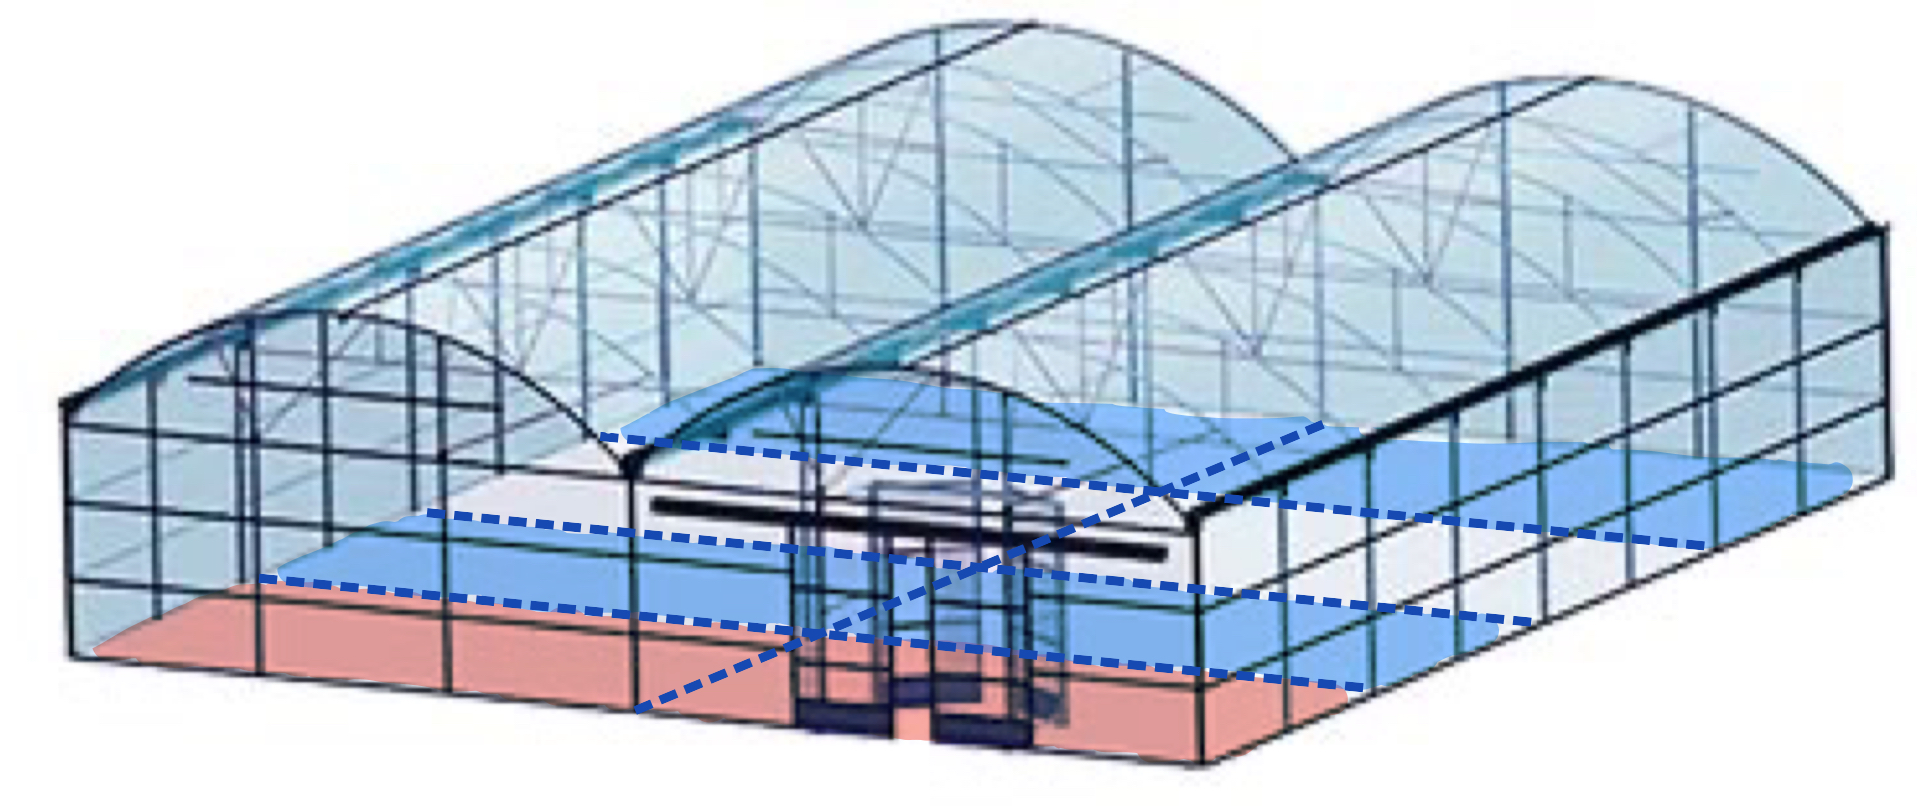
\includegraphics[width=\textwidth]{img/05-InvernaderoCapilla-Base.jpeg}
    \captionof{figure}{Dibujo de un invernadero tipo capilla (Novagric)}
    \label{fig:invernadero_capilla}
\end{center}

En base al dibujo anterior se va a plantear la división del terreno en 8 cuadrantes, mostrado con una vista aérea en el siguiente diagrama \ref{fig:invernadero_base}:

\begin{center}
    \centering
    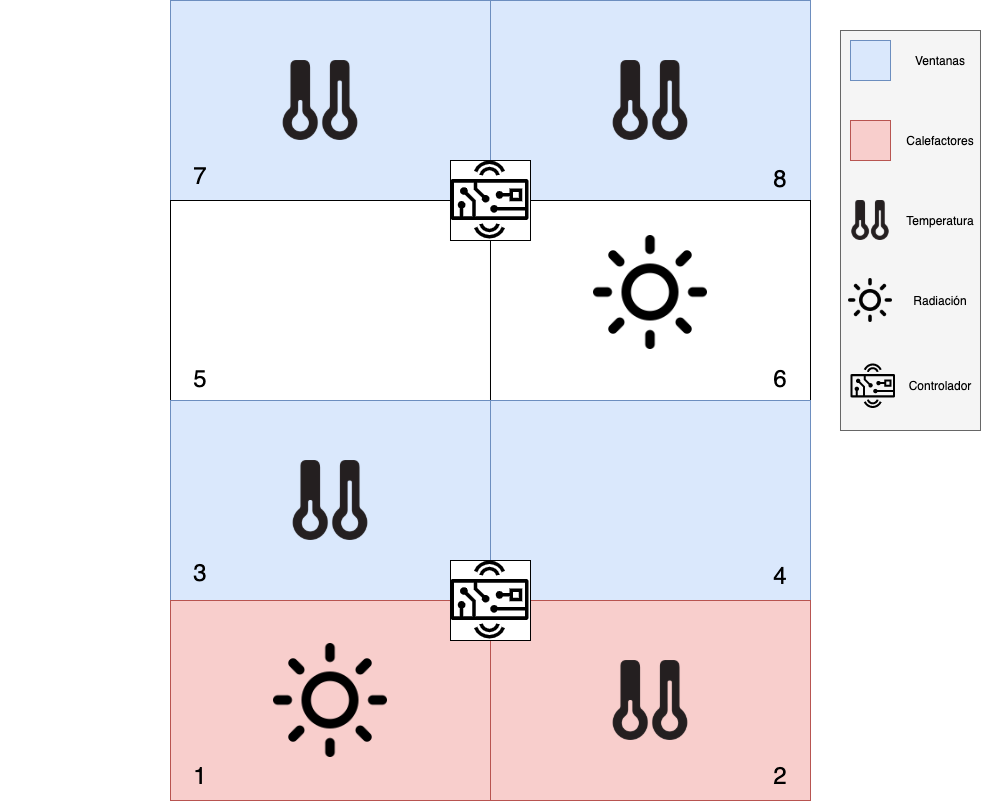
\includegraphics[width=\textwidth]{img/04-Invernadero_base.png}
    \captionof{figure}{Diagrama de un invernadero con vista aérea}
    \label{fig:invernadero_base}
\end{center}

Hay una leyenda en la figura indicando que es cada dispositivo, aclarando en la siguiente lista su funcionamiento:

\begin{itemize}
    \item \textbf{Sensor de temperatura.} Sensores situados en las zonas 2, 3, 7 y 8. Publica los datos recopilados.
    \item \textbf{Sensor de radiación.} Sensor situado en las zonas 1 y 6. Publica los datos recopilados.
    \item \textbf{Ventanas.} Cada recuadro azul indica que hay motores de ventanas en esa zona, como los mostrados en la figura \ref{fig:imagenes-actuadores}
    \item \textbf{Calefacción.} Cada recuadro rojizo hace referencia a la zona de actuación de los calefactores. En función de los datos suministrados por el sensor de temperatura 1 se activa o desactiva.
    \item \textbf{Controlador.} Encargado de recoger los distintos datos.
\end{itemize}

Además de estos dispositivos, hay un gestor de la base de datos para almacenar los datos recogidos por los controladores y una interfaz web. Estos no se han incluido en el escenario porque pueden estar desplegados en otro lugar.


\section{Diseño de clases de cada dispositivo}

Cada nodo mostrado como se ha podido ver durante el análisis dispone de diferentes conexiones y funciones a realizar, las cuales se van a ver reflejadas en la esta sección:

\begin{center}
    \centering
    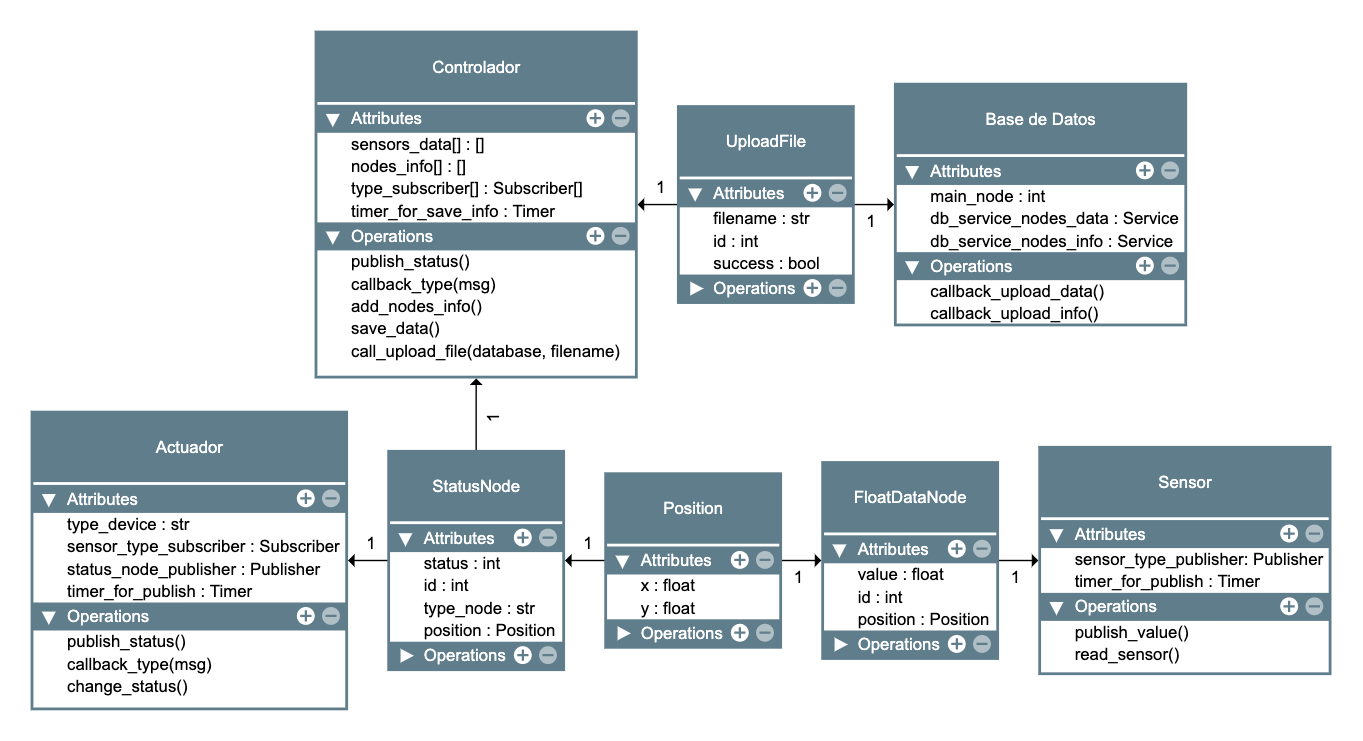
\includegraphics[width=\textwidth]{img/05-DiagramaClasesCompleto.png}
    \captionof{figure}{Diagrama de clases}
    \label{fig:diagrama-clases}
\end{center}

En este diagrama están representados los sensores y actuadores de manera genérica. En función del número de datos que recopile un sensor, existirá el mismo número de \textit{publicadores} o \textit{publishers}. Y en el caso de los datos necesarios por un actuador para realizar alguna acción, habrá ese mismo número de suscriptores.

Además en el caso del controlador, en el array mostrado \textit{type\_subscriber}, tendrá uno por cada tópico diferente en la red.

Las clases UploadFile, StatusNode, Position y FloatDataNode son autogeneradas a partir de un archivo por ROS2, por lo tanto están mostradas en la figura \ref{fig:estructuras-interfaces} de la siguiente sección.

\section{Diseño de interfaces en ROS2}

En esta sección se va a tratar la parte de comunicación entre los diferentes nodos. Para ello se tienen que definir las estructuras a utilizar para la comunicación, ya que es necesario indicar el tipo de mensaje a utilizar.

Un tópico \cite{topic} representa la unidad de información que puede ser producida o consumida por una aplicación DDS. ROS 2 las renombra interfaces debido a que las utiliza para comunicación publicador-suscriptor y cliente-servidor.

En el siguiente diseño se muestran las diferentes estructuras utilizadas.

\begin{center}
    \centering
    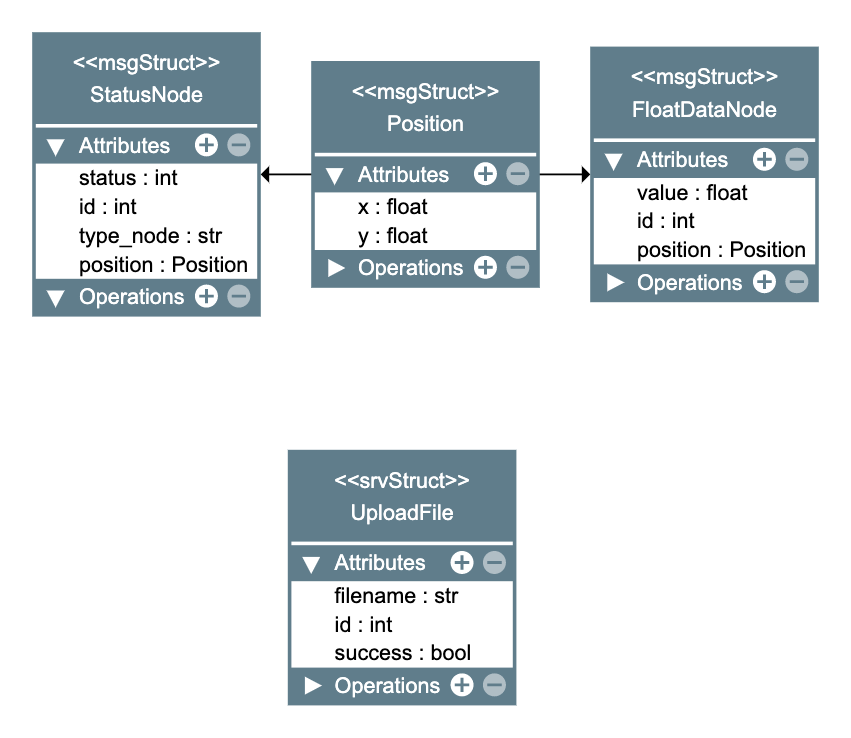
\includegraphics[width=\textwidth]{img/05-Interfaces.png}
    \captionof{figure}{Estructuras definidas utilizadas en los tópicos}
    \label{fig:estructuras-interfaces}
\end{center}

Estas estructuras en DDS se definen en archivos \ac{IDL}, los cuales definen una estructura estandarizada para todas las arquitecturas contempladas, y a partir de ella son generados los diferentes ficheros necesarios para utilizarlos como tipo de mensaje en un tópico. En ROS2 son conocidas como interfaces, subdivididas en dos grupos, los servicios y los mensajes. Estos pueden ser visualizados en las cabeceras de la figura anterior, explicadas a continuación:

\begin{itemize}
    \item \textbf{msgStruct}, hace referencia a un mensaje, utilizado de forma pub-sub en un tópico.
    \item \textbf{srvStruct}, hace referencia a un servicio, utilizado en una conexión cliente-servidor. Esta conexión se utiliza en la comunicación del Controlador y el gestor de la Base de Datos.
\end{itemize}

Ahora se van a analizar las diferentes interfaces utilizados en este despliegue, los cuales llevan asociado un tipo del conjunto anterior.

\begin{center}
    \centering
    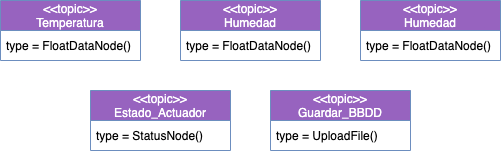
\includegraphics[width=\textwidth]{img/05-Topicos.png}
    \captionof{figure}{Interfaces}
    \label{fig:topicos}
\end{center}

Como podemos observar, existen 5 tipos de interfaces, 4 de ellas referentes a los nodos mostrados en el esquema \ref{fig:invernadero_base}, y otra referente al almacenamiento de los datos.

Cada uno de estos interfaces tienen asociadas un conjunto de \ac{QoS}, utilizados en ROS2 \cite{qos-ros}. QoS hace referencia a unas políticas de comunicación que se pueden establecer entre los nodos. En la siguiente lista se van a explicar las más destacables para este proyecto:

\begin{itemize}
    \item \textit{Keep last}, haciendo referencia al número de datos a almacenar en la cola, ya que si no se podrían almacenar todos.
    \item \textit{Queue size}, valor utilizado en \textit{keep last} si está asignado
    \item \textit{Reliable}, para asegurar que los datos lleguen a su destino
    \item \textit{Volatile}, no se hace intento de hacer persistentes las muestras.
\end{itemize}

Para finalizar esta sección, se va a mostrar un diagrama de comunicación entre los diferentes nodos, pudiendo observar como operan con los tópicos en la red.

Por aclarar, los diferentes nodos están mostrados con óvalos, y en el caso de los tópicos, se utilizan los rectángulos.

\begin{landscape}
\begin{figure}
    \centering
    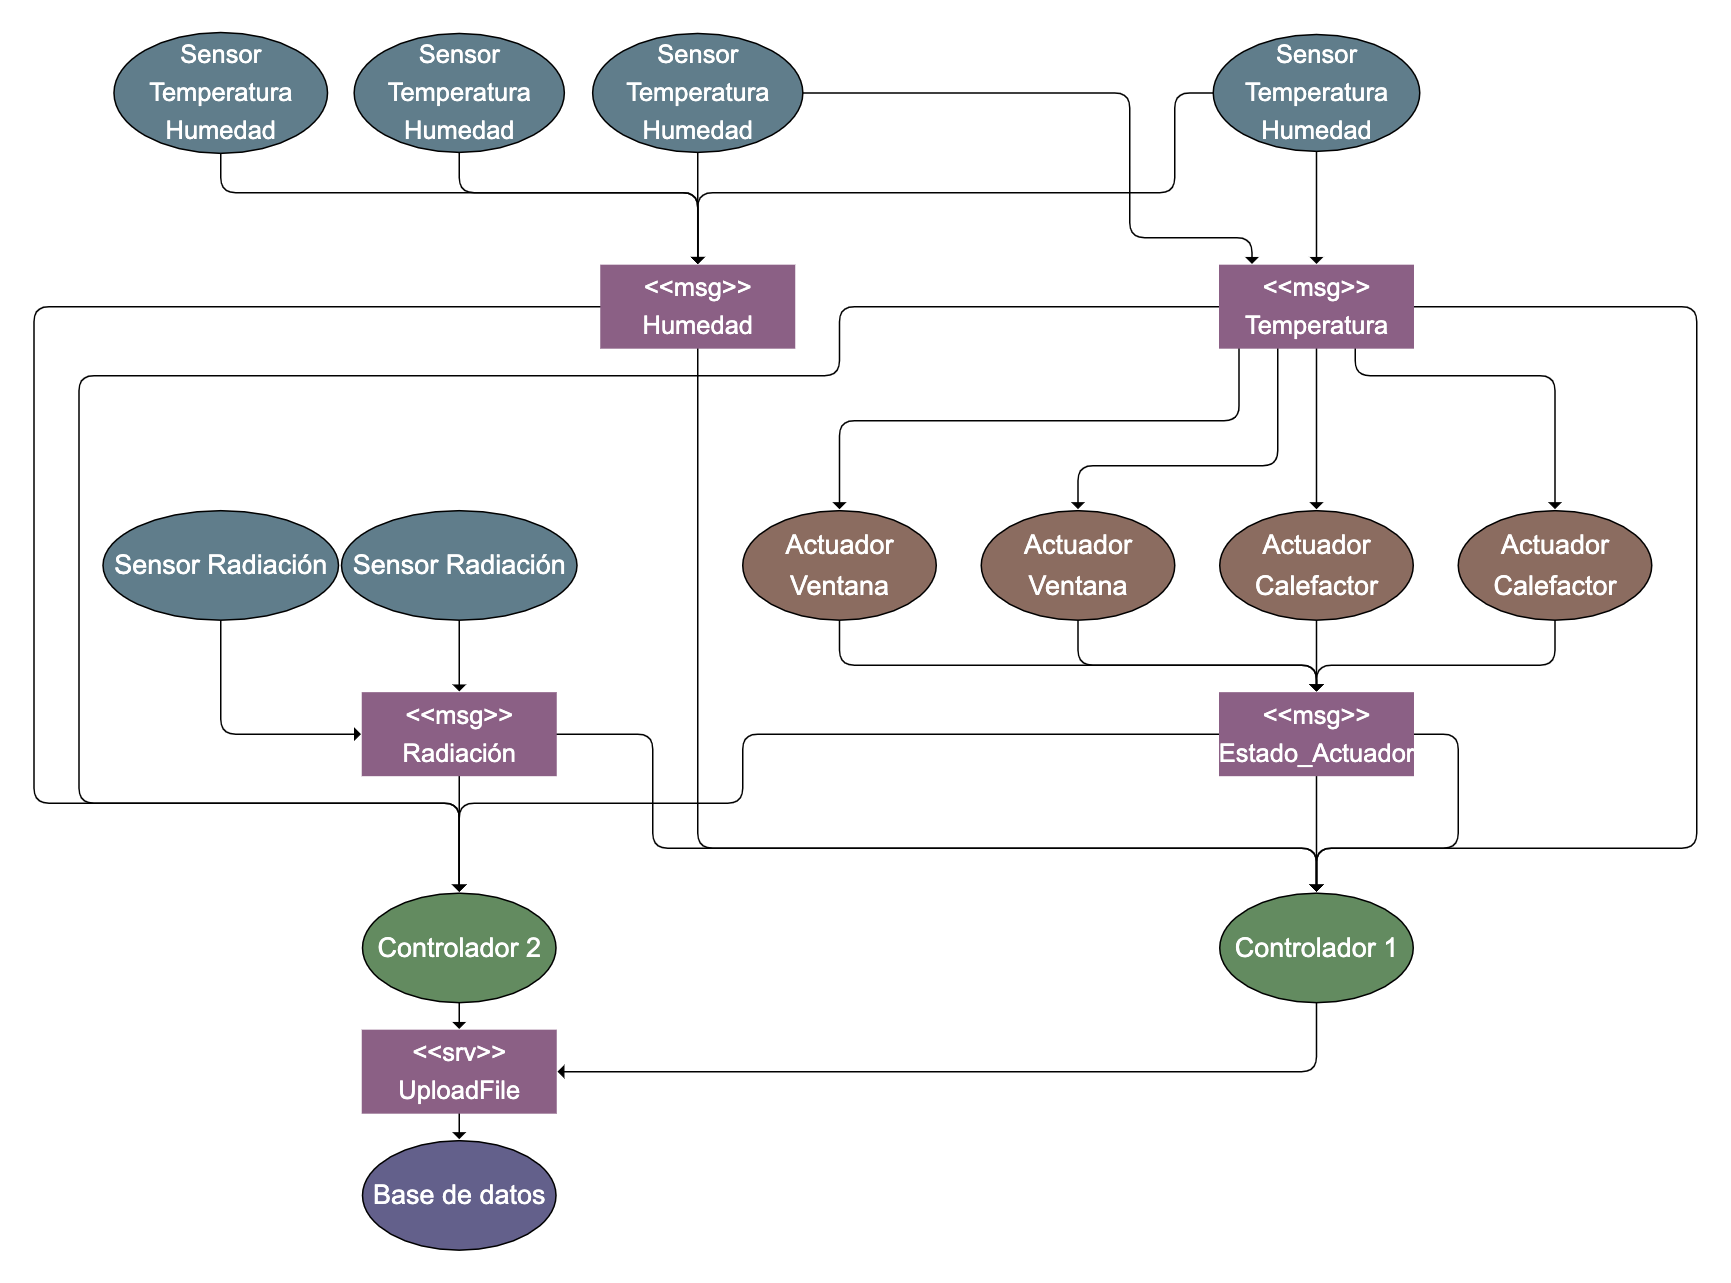
\includegraphics[width=1.6\textwidth]{img/05-DiagramaComunicacion.png}
    \caption{Diagrama de comunicación entre nodos}
    \label{fig:diagrama-comunicacion-nodos}
\end{figure}
\end{landscape}


\section{Diseño de la Base de Datos}

Tras las explicaciones de los datos tratados en las secciones anteriores, es necesario esquematizar que datos se van a guardar y como van a ser distribuidos. Para ello se van a definir dos tablas principales: sensores y actuadores. Estos deberán constar de los siguientes componentes:

\begin{itemize}
    \item \textbf{Id}. Almacena el id del dispositivo
    \item \textbf{Tipo}. Almacena el tipo de dato producido
    \item \textbf{Posición}. Almacena la posición del nodo
\end{itemize}

Aquí no se incluye ningún valor registrado sobre el estado del nodo o que valor esta obteniendo de los sensores, si no información más relacionada con su tipo o localización, información que varia poco a lo largo del tiempo. 

Únicamente va a existir una entrada por cada Id definido en la tabla. En el caso de que llegue nueva información por si el dispositivo se ha modificado su ubicación, o si transmite nuevos tipos de datos, esta entrada será actualizada.

Por otro lado, se va a tener una tabla por cada tipo de medida (temperatura, humedad...) y tipo de actuador (ventana, calefacción...). La estructura definida para este caso es:

\begin{itemize}
    \item \textbf{Id}. Id del dispositivo
    \item \textbf{Valor}. Valor recogido por el sensor, o estado del actuador
    \item \textbf{Timestamp}. Tiempo haciendo referencia a cuando se ha enviado este dato por la red.
\end{itemize}

Un ejemplo de tabla de \textit{Temperatura} con algunos datos seria la siguiente:

\begin{center}
\begin{tabular}{||c c c||} 
 \hline
 Id & Valor & Timestamp \\ [0.5ex] 
 \hline\hline
 11 & 23 & "10/26/21, 11:30:15" \\ 
 \hline
 12 & 21 & "10/26/21, 11:30:15" \\
 \hline
 13 & 20 & "10/26/21, 11:30:15" \\
 \hline
 11 & 22 & "10/26/21, 11:15:20" \\ 
 \hline
 12 & 21 & "10/26/21, 11:15:20" \\


 \hline
\end{tabular}
\captionof{figure}{Tabla de Temperatura}
\end{center}

En este caso se añade una entrada a la tabla por cada muestra obtenida, para luego poder visualizar los datos a lo largo del tiempo.


\section{Diseño de la interfaz web}

Esta es la parte final del capítulo, ya que tras analizar diseño a implementar, es necesario que el cliente pueda observar todos estos datos. Para ello se ha planteado un entorno web adaptable a distintos dispositivos desde donde se pueda interactuar para consultar información o mandar órdenes al sistema.

Este debe poder acceder a la base de datos mencionada anteriormente, y mostrar los datos en diferentes categorías.

La web debería constar de los siguientes componentes:

\begin{center}
    \centering
    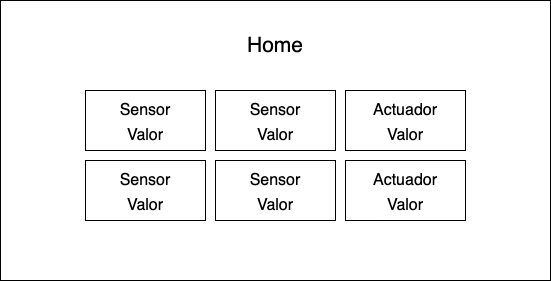
\includegraphics[width=\textwidth]{img/05-Web-home.png}
    \captionof{figure}{Página principal}
    \label{fig:home}
\end{center}

La página principal será la primera pantalla de la interfaz, donde se muestra en un dashboard el valor o estado actual de los diferentes nodos que hay desplegados en el escenario, pudiendo ver de un vistazo la información.

\begin{center}
    \centering
    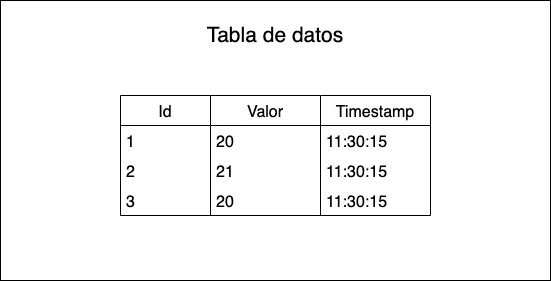
\includegraphics[width=\textwidth]{img/05-Web-tablas.png}
    \captionof{figure}{Tablas de datos}
    \label{fig:tablas-de-datos}
\end{center}

La figura anterior \ref{fig:tablas-de-datos} muestra todos los datos recopilados en la base de datos, subdivididas según el tipo de dato (temperatura, humedad..). Además sería conveniente poder buscar algún valor por hora, filtrar por id o incluso ordenar por parámetros.

\begin{center}
    \centering
    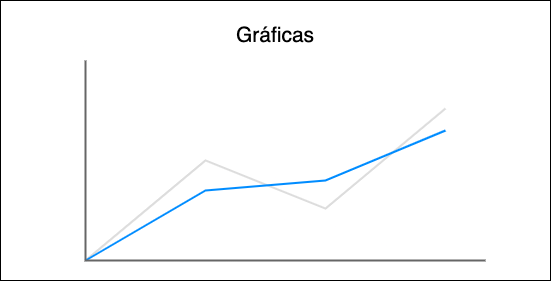
\includegraphics[width=\textwidth]{img/05-Web-charts.png}
    \captionof{figure}{Gráficas}
    \label{fig:graficas}
\end{center}

Sería idónea la implementación de una sección con los diferentes datos mostrados en gráficas, ya que facilita al usuario la interpretación y la visualización de la información respecto al tiempo, pudiendo comparar los diferentes sensores de una forma más sencilla.

 Además es complicado recordar que nodo esta situado en cada posición, por lo que un mapa con cada uno situado sería una funcionalidad a considerar. Esto vendría a ser similar a la figura \ref{fig:invernadero_base}. Para visualizarlo al igual que los ejemplos anteriores, se adjunta una imagen \ref{fig:mapa} a continuación del diseño planteado:
 
 \newpage
 
 \begin{center}
    \centering
    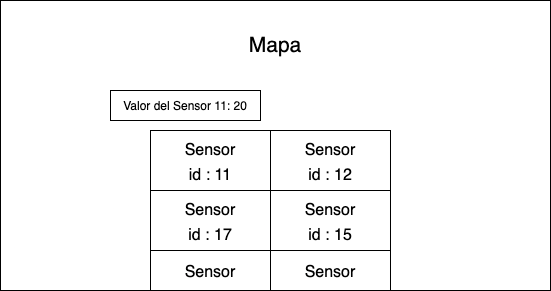
\includegraphics[width=\textwidth]{img/05-Web-map.png}
    \captionof{figure}{Mapa para visualizar la localización de los componentes}
    \label{fig:mapa}
\end{center}

Una funcionalidad interesante a implementar sería que seleccionar un sensor, el apartado de \textit{Valor del sensor} se actualice y muestre el estado actual de este.